\documentclass[titlepage]{article}
\usepackage[english]{babel}
\usepackage[letterpaper, top=2.5cm, bottom=2.5cm, left=2.5cm, right=2.5cm, marginparwidth=1.75cm]{geometry}

\usepackage{amsmath,amsthm,amssymb}
\usepackage{bbold}
\usepackage{graphicx}
\usepackage{listings}
\usepackage{multicol}
\usepackage{setspace}
\usepackage{enumitem}
\usepackage{float}
\usepackage{apacite}
\usepackage{xcolor}

\usepackage{tikz}
\usetikzlibrary{arrows.meta, positioning}

% Common set symbols
\newcommand{\Z}{\mathbb{Z}}
\newcommand{\N}{\mathbb{N}}
\newcommand{\R}{\mathbb{R}}
\newcommand{\Q}{\mathbb{Q}}
\newcommand{\C}{\mathbb{C}}
\newcommand{\B}{\mathbb{B}}
\newcommand{\nullset}{\varnothing}
\newcommand{\powerset}[1]{\mathcal{P} ({#1})}
\newcommand{\ol}[1]{\overline{#1}}

\newcommand{\divides}{\mid}
\newcommand{\notdivides}{\nmid}

\newcommand{\st}{\text{ such that }}
\newcommand{\pmi}{\text{ principle of mathematical induction }}

\newcommand{\editnote}[1]{\textcolor{red}{{#1}}}
\newcommand{\nitem}[1] % sets enumerate to a specific number {arg1}
{
    \setcounter{enumi}{#1}
    \addtocounter{enumi}{-1}
    \item
}
\usepackage{multicol}
\newtheorem{theorem}{Theorem}[section]
\newtheorem{lemma}{Lemma}[section]
\title{Math 418\\ \large Synthetic Handwriting with Generative Adversarial Networks}
\author{
    Micah Sherry \\
    \texttt{nbzx@iup.edu}
}

\begin{document}

\maketitle

\section{Introduction}

The goal of this research project is to use a Generative Adversarial Neural Network (GAN)\editnote{add citation} to create synthetic handwritten letters.
Generative models have become an important area of machine learning due to their ability to learn complex data distributions and generate realistic samples that resemble real-world data.
In particular, GANs have shown strong performance in generating high-quality images by training two neural networks in opposition: a generator that creates synthetic data and a discriminator that attempts to distinguish between real and generated samples. Below is a simplfied illustration of a conditional GAN model

\begin{figure}[h]
    \centering
    \resizebox{0.95\linewidth}{!}{
    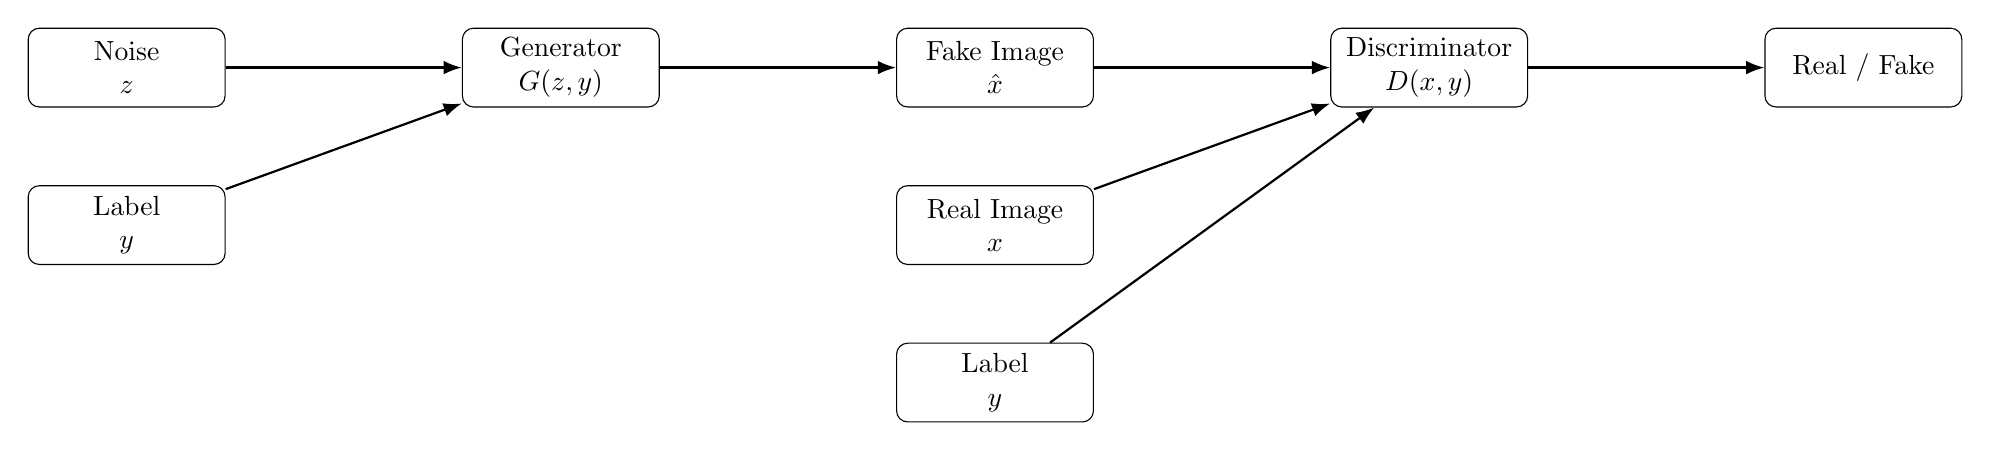
\begin{tikzpicture}[
        node distance=2cm,
        box/.style={draw, rounded corners, align=center, minimum width=2.5cm, minimum height=1cm},
        arrow/.style={-Latex, thick}
    ]
    
    % Nodes
    \node[box] (noise) {Noise \\ $z$};
    \node[box, below of=noise] (label1) {Label \\ $y$};
    
    \node[box, right=3cm of noise] (gen) {Generator \\ $G(z,y)$};
    \node[box, right=3cm of gen] (fake) {Fake Image \\ $\hat{x}$};
    
    \node[box, below of=fake] (real) {Real Image \\ $x$};
    \node[box, below of=real] (label2) {Label \\ $y$};
    
    \node[box, right=3cm of fake] (disc) {Discriminator \\ $D(x,y)$};
    \node[box, right=3cm of disc] (out) {Real / Fake};
    
    % Arrows - Generator
    \draw[arrow] (noise) -- (gen);
    \draw[arrow] (label1) -- (gen);
    \draw[arrow] (gen) -- (fake);
    
    % Arrows - Discriminator (fake path)
    \draw[arrow] (fake) -- (disc);
    
    % Arrows - Discriminator (real path)
    \draw[arrow] (real) -- (disc);
    \draw[arrow] (label2) -- (disc);
    
    % Output
    \draw[arrow] (disc) -- (out);
    
    \end{tikzpicture}
    }
    \caption{Conditional GAN (cGAN) architecture}
    \label{fig:cgan}
    \end{figure}

In this project, the GAN is trained on the EMNIST Balanced dataset \editnote{add citation}, which is an extension of the MNIST dataset containing both handwritten digits and letters. The dataset consists of 47 distinct classes: 10 classes representing the digits 0 to 9, and 37 classes representing uppercase and lowercase letters. Some letter classes were merged due to visual similarity, making classification more consistent and reducing ambiguity between certain character pairs.

The EMNIST Balanced dataset presents a more challenging task than standard digit recognition because of the increased number of classes and the variability in handwritten letter shapes. This makes it a suitable benchmark for evaluating the performance of generative models in learning complex character distributions.

Below is an image illustrating the distribution of samples across the different classes in the dataset:

\begin{figure}[h]
    \centering
    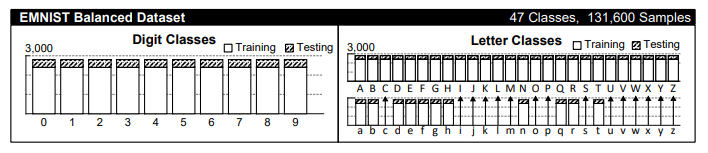
\includegraphics[width=0.8\textwidth]{images/dataset_breakdown.png}
    \caption{Class distribution of the EMNIST Balanced dataset}
    \label{fig:dataset_breakdown}
\end{figure}

The objective of this work is not only to generate visually realistic handwritten characters but also to evaluate the quality of the generated samples using a trained classifier. By analyzing classification accuracy on synthetic data, we aim to measure how well the generator has learned the underlying structure of the dataset.

\section{Traditional GAN}
The first area of investigation was whether a GAN model without convolutional layers could be trained. We expect that this model will not perform well due to the highly complex and spatially structured nature of handwritten characters. Unlike convolutional architectures, fully connected layers do not preserve spatial relationships between pixels, making it difficult for the model to learn meaningful local patterns such as strokes and curves that are essential for realistic handwritten character generation.

\subsection{Training Details}
The conditional Generative Adversarial Network (cGAN) was trained using the EMNIST Letters dataset, which consists of handwritten characters spanning 26 alphabet classes. The dataset images were normalized to the range $[-1, 1]$ and reshaped to $28 \times 28 \times 1$ grayscale format.

The training process was conducted for a total of 200 epochs. The dataset contains approximately 62400 training images, which were shuffled and divided into batches of size 128 during training. 

During each training step, the generator receives a random noise vector of dimension 100 concatenated with a class label, and attempts to generate realistic handwritten character images. The discriminator is trained simultaneously to distinguish between real and generated images conditioned on the same class labels.

The training was performed using the Adam optimizer with a learning rate of $2 \times 10^{-4}$. The adversarial loss was computed using binary cross-entropy for both the generator and discriminator networks.

To monitor progress, sample images for all 26 classes were generated every 5 epochs.
\subsection{Results}
The result of training a GAN model without convolutional layers provided  unusable synthetic handwritten images.  Figure~\ref{fig:gan_wo_conv} shows synthetic images generate after training for 200 epochs. Notice that all the images are highly similar to each other and do not resemble any letter. 

\begin{figure}[h]
    \centering
    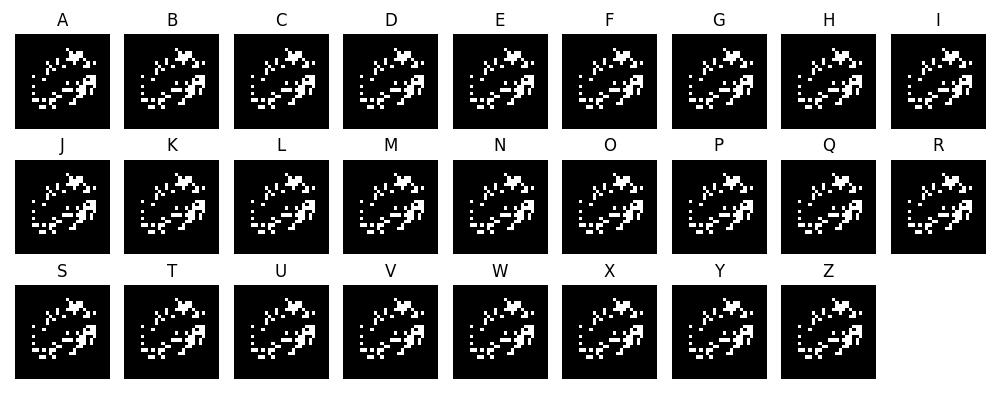
\includegraphics[width=0.8\textwidth]{images/regular/train_200.png}
    \caption{Synthetic Images Generated by GAN without Convolutional Layers}
    \label{fig:gan_wo_conv}
\end{figure}
 

\section{GAN With Convolutional Layers}
Now that we know that GAN with traditional neural network layers does not perform well with this dataset. We now look at GAN with convolutional layers.
Convolutional layers have proven to be a good choice for neural networks for image processing because allow the model to better detect local features and spacial relationships such as edges, corners, and curves which is extremely important to image classification.   

\subsection{Training Details}
The training process was very similarity to the model without convolutional layers. 

The model was trained using the EMNIST Balanced dataset, which consists of handwritten characters across 47 classes. The dataset images were normalized to the range $[-1, 1]$ and reshaped to $28 \times 28 \times 1$ grayscale format.

The training process was conducted for a total of 100 epochs. The dataset contained approximately 112,800 training images, which were shuffled and divided into batches of size \textbf{128} during training.

During each training step, the generator receives a random noise vector of dimension 100 concatenated with a learned class label embedding and produces synthetic handwritten character images. The discriminator receives both real and generated images, along with their corresponding class labels, and learns to classify them as real or fake.

The generator architecture is based on convolutional transpose layers, which progressively upsample the input vector into a $28 \times 28$ image. The discriminator uses convolutional layers to extract hierarchical spatial features before performing binary classification.

The model was trained using the Adam optimizer with a learning rate of $2 \times 10^{-4}$ and $\beta_1 = 0.5$. Binary cross-entropy was used as the adversarial loss function for both the generator and discriminator networks.

To monitor training progress, sample images for all 47 classes were generated every 5 epochs and saved for qualitative evaluation.

\subsection{Results}
As expected the model with convolutional layers performed very well (compared to traditional model). Even after 5 epochs the generated images(See Figure~\ref{fig:epoch5}) are useable. And after 100 epochs the images (See Figure~\ref{fig:epoch100}) appear very closely like handwritten characters.   
\begin{figure}[h]
    \centering
    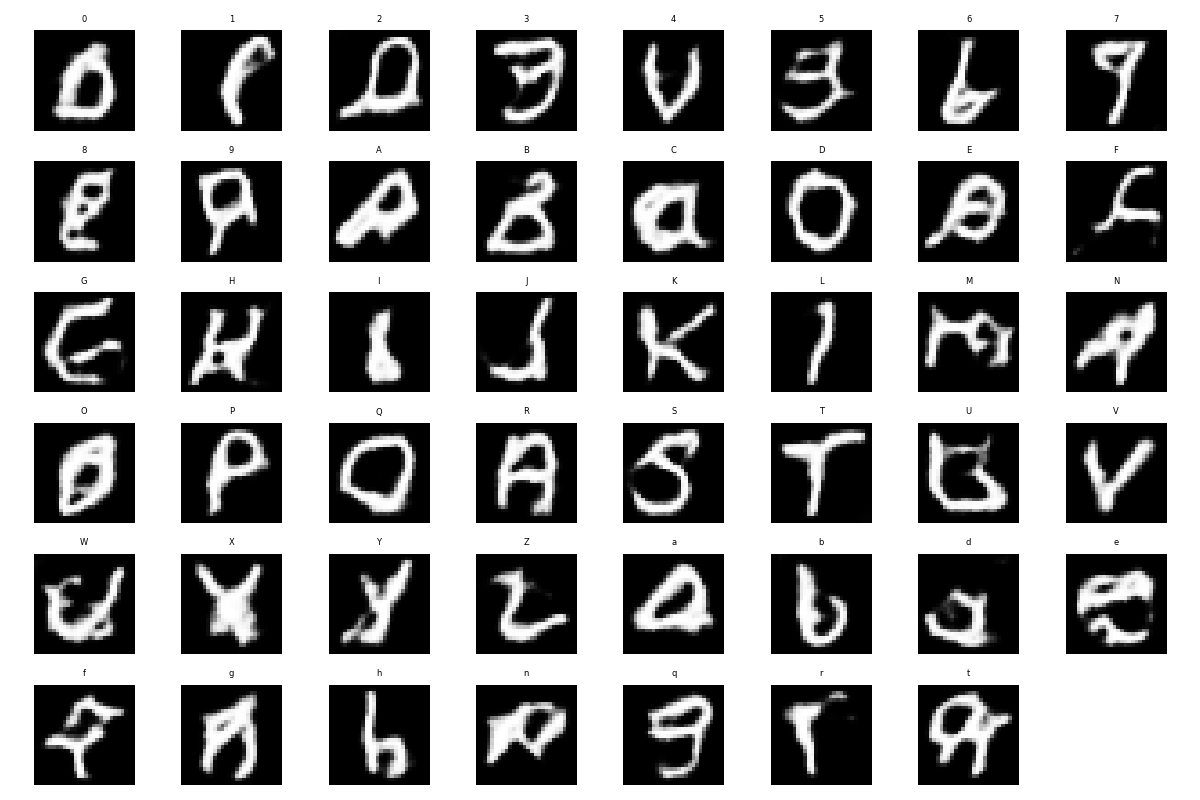
\includegraphics[width=0.8\textwidth]{images/conv/epoch_5.png}
    \caption{Synthetic images generated by GAN with Convolutional layers after 5 epochs}
    \label{fig:epoch5}
\end{figure}
\begin{figure}[h]
    \centering
    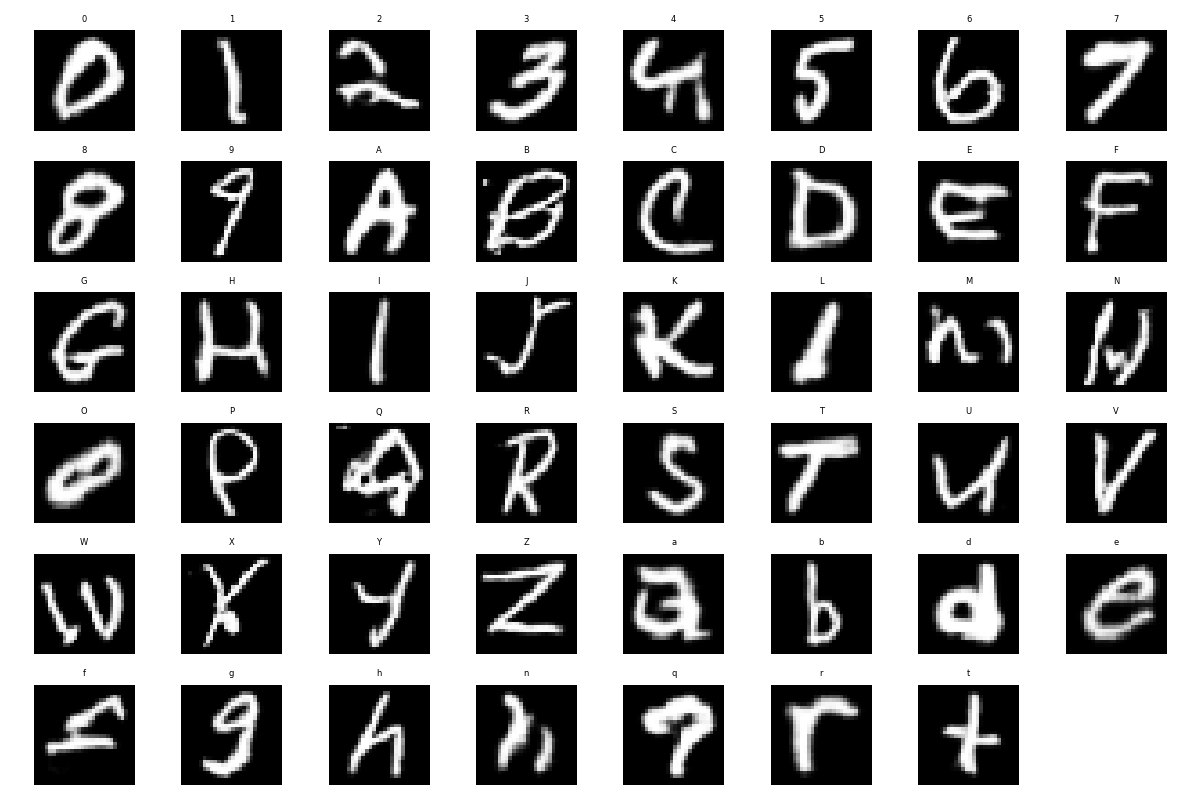
\includegraphics[width=0.8\textwidth]{images/conv/epoch_100.png}
    \caption{Synthetic images generated by GAN with Convolutional layers after 100 epochs}
    \label{fig:epoch5}
\end{figure}
 

\section{Benchmarking}
Determining how well the model performs is difficult because of the subjectivity of Determining images looks better. 

\subsection{Classification Model}
To get a Numerical Score of how well a model performed a classification model was trained on the EMNIST Balanced dataset. Then the generator was used to create a synthetic dataset. the Synthetic dataset was then scored on classification accuracy. Figure~\ref{fig:class} shows classification accuracy of the synthetic dataset by epoch

\begin{figure}[h]
    \centering
    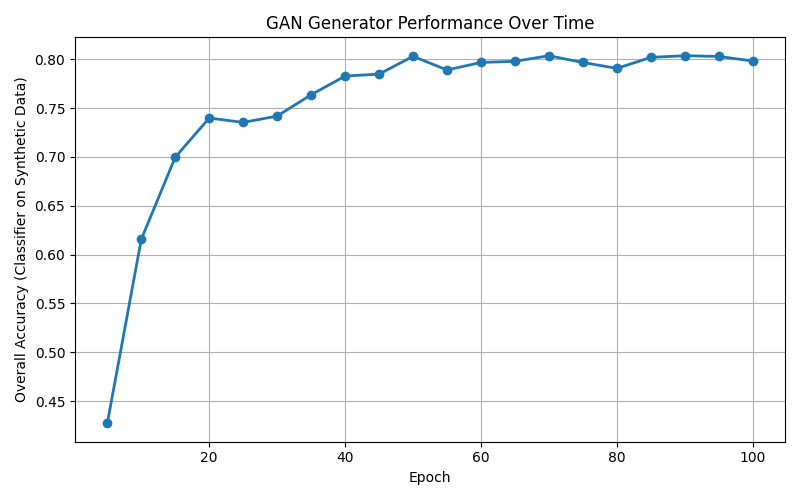
\includegraphics[width=0.8\textwidth]{images/accuracy_by_epoch.png}
    \caption{classification accuracy by epoch}
    \label{fig:class}
\end{figure}



\end{document}